%-------------------------
%big-picture
%(c) H.Buchmann FHNW 2008
%$Id$
%export TEXINPUTS=${HOME}/fhnw/edu/:${HOME}/fhnw/edu/tinL/config/latex:${HOME}/fhnw/edu/config//:
%-------------------------
\documentclass{beamer}
\usepackage{latex/beamer}
%---------------------
%local defines
%(c) H.Buchmann FHNW 2009
%$Id$
%---------------------
\newcommand{\target} {\beaglebone\xspace}
\newcommand{\targetS}{{\bf BBG}\xspace}
\newcommand{\host}   {{\em Host}\xspace}
\newcommand{\targetroot} {{\bf target-root}\xspace}
\newcommand{\kernel} {{\bf kernel}\xspace}
\renewcommand{\c}{{\bf C}\xspace}
\newcommand{\cpp}{{\bf C++}\xspace}
\newcommand{\posix}{{\bf POSIX}\xspace}


\title[\unix use]{\unix use}
\begin{document}

\frame{\titlepage}

\begin{frame}{Ziel}{Entwicklung von Programmen auf dem \target}
 \begin{itemize}
  \item alles ist ein File 
  \begin{itemize}
   \item $0-te$ Näherung
   \item File: {\em stream of bits}
  \end{itemize}
  \item Filesysteme
  \begin{itemize}
   \item \cod{mount}
   \item \cod{sshfs}
  \end{itemize}
  \item Cross development
  \begin{itemize}
   \item \host $\leftrightarrow$ \target
   \remark{Keine Toolchain auf dem \target}
  \end{itemize}
 \end{itemize}
\end{frame}

\begin{frame}{Wichtig}
 \begin{itemize}
  \item wo ist was ?
  \begin{itemize}
  \item {\Large Verzeichnisstruktur}
  \end{itemize}
  \item wo sind wir ?
  \begin{itemize}
   \item \host
   \item[] oder
   \item \target
  \end{itemize}
 \end{itemize}
\end{frame}

\section{Alles ist ein File}
\begin{frame}{Alles ist ein File}{stream of bits}
 \begin{center}
  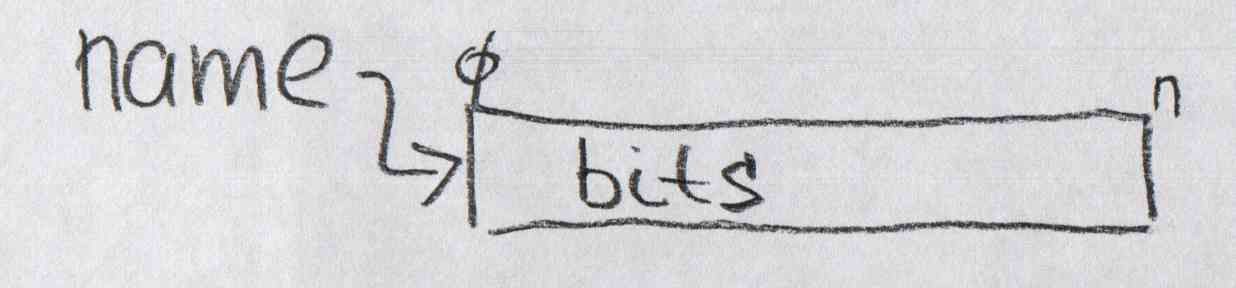
\includegraphics[width=0.5\textwidth]{file-bits.jpg}
 \end{center}
 \begin{itemize}
  \item \cod{\em name} Referenz auf die Bits (Bytes)
  \begin{itemize}
   \item Bits(bytes) der Reihe nach
   \item indexiert $0\dots n-1$
  \end{itemize}
  \item File
  \begin{itemize}
   \item Datenquelle
   \begin{itemize}
	\item liefert Daten: Bits(Bytes)
   \end{itemize}
   \item Datensenke
   \begin{itemize}
	\item absorbiert Daten: Bits(Bytes)
   \end{itemize}
  \end{itemize}
 \end{itemize}
\end{frame}

\begin{frame}{Ein paar Befehle}
 \begin{itemize}
  \item \cod{cat {\em name}} 
  \begin{itemize}
   \item {\em concatenate files and print on the standard output}
   \item zeigt den Inhalt
  \end{itemize}
  \item \cod{hexdump -C {\em name}}
  \begin{itemize}
   \item {\em display  file  contents  in hexadecimal, decimal, octal, or ascii}
   \item zeigt die Bits hexadezimal
  \end{itemize}
  \item \cod{dd if=... of=... count=...}
  \begin{itemize}
   \item {\em convert and copy a file}
   \item brauchen wir oft
  \end{itemize}
 \end{itemize}
\end{frame}

\subsection{Devices}
\begin{frame}{Devices sind auch Files}{am Beispiel SD-Karte}
 \begin{description}
  \item[\cod{/dev/mmcblk{\bf i}}] $i=0,1,2 ...$
  \remark{Name vom Betriebssystem bestimmt}
  \begin{description}[Datenquelle]
  \item[Datenquelle] \cod{hexdump -C /dev/mmcblk0}
  \item[Datensenke] \cod{cp {\em name} /dev/mmcblk0}
  \remark{Aufpassen}
  \end{description}
 \end{description}
\end{frame}

\begin{frame}{Devices sind auch Files}{z.B Zufallszahlen}
 \begin{description}[\cod{/dev/urandom}]
  \item[\cod{/dev/random}] sammelt das Rauschen: langsam
  \remark{Name vom Betriebssystem bestimmt}
  \begin{description}
   \item[Datenquelle] \cod{hexdump -C /dev/random}
  \end{description}
  \item[\cod{/dev/urandom}] berechnete (Pseudo) Zahlen: schnell
  \begin{description}
   \item[Datenquelle]
   \cod{play -b 16 -e  signed-integer  \textbackslash\\
   -t raw -r 44000 /dev/urandom}
   \remark{der Befehl \cod{play} hat viele Optionen}
  \end{description}
 \end{description}
\end{frame}

\section{Filesystem}
\begin{frame}{Filesystem}{Files für Files}
 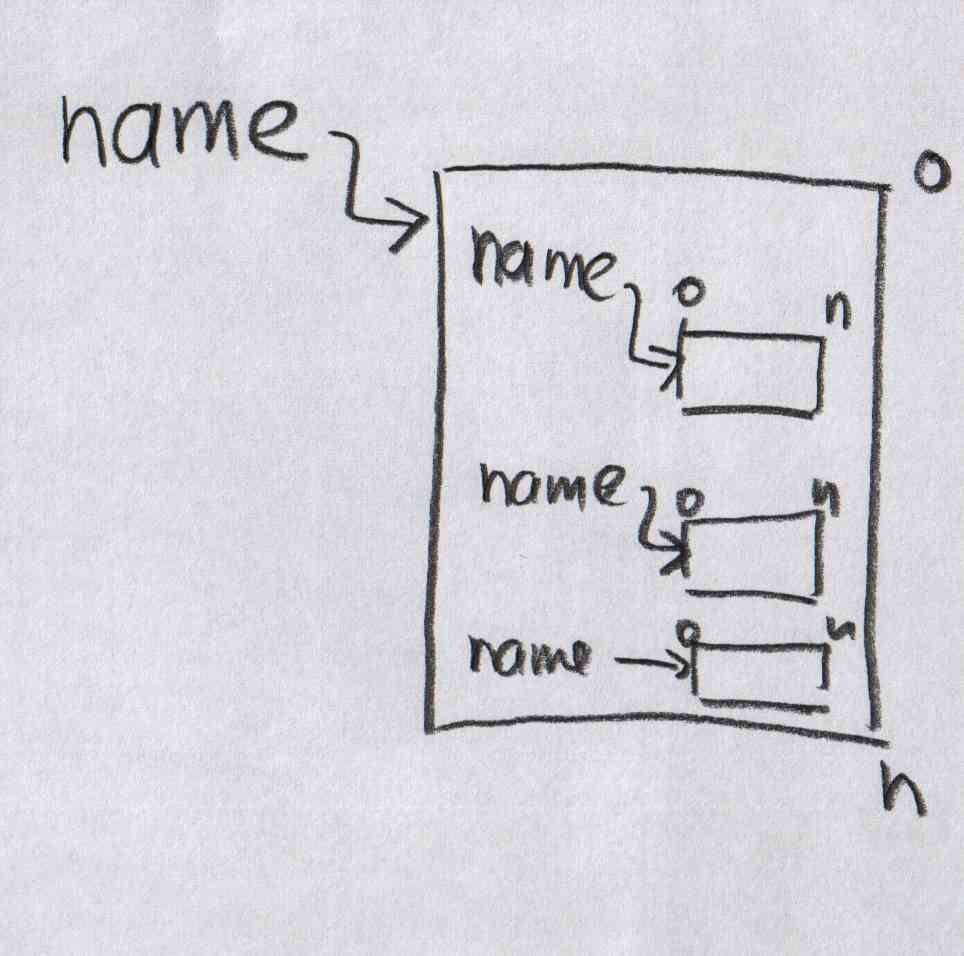
\includegraphics[width=4.5cm]{filesystem.jpg}
 \begin{textblock}{150}(55,30)
  \begin{itemize}
   \item File der weitere Files enthält
   \item Verschiedene Filesysteme
   \begin{description}
    \item[vfat] Microsoft 
    \item[ext4] \unix
    \item[...] noch viele andere \\\cod{cat /proc/filesystems}
   \end{description}
  \end{itemize}
 \end{textblock}
\end{frame}

\begin{frame}{Vereichnisstruktur}{Hierarchie}
 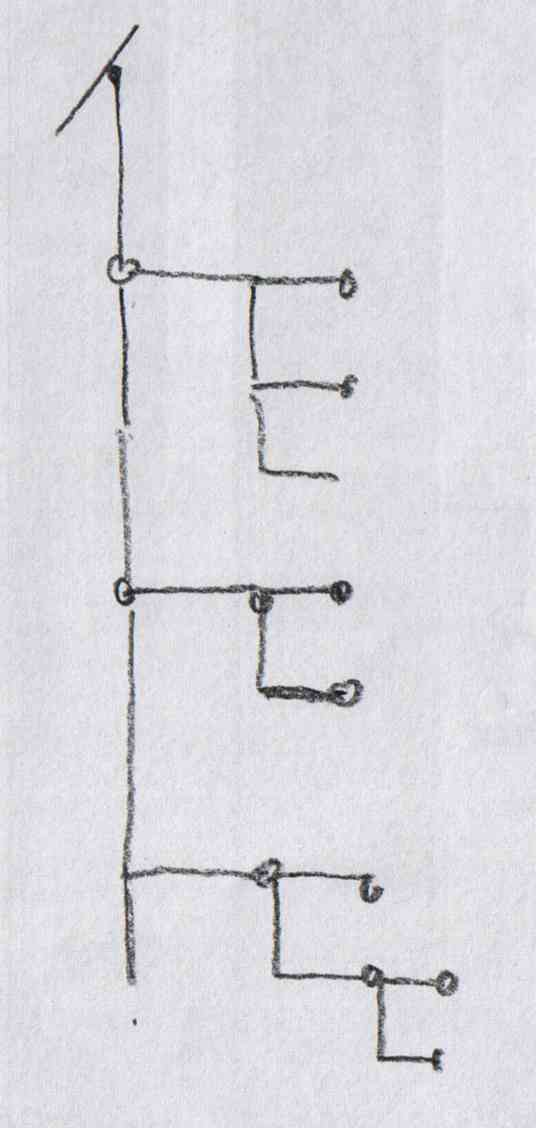
\includegraphics[height=5cm]{dir-tree.jpg}
 \includegraphics[height=5cm]{glbs/2-as-user/doc/tree.png}
 \begin{textblock}{150}(80,65)
  \begin{itemize}
   \item \cod{/} root
   \item ein paar Befehle 
   \begin{itemize}
   \item \cod{ls}, \cod{tree}, \cod{cd}
   \end{itemize}
  \end{itemize}
 \end{textblock}
 \hint[30]{50,40}{Verzeichnisse einer Workstation}
\end{frame}


\begin{frame}{\cod{mount {\em fileSystem} {\em mountPoint}}}
             {Verbindet Filesysteme}
  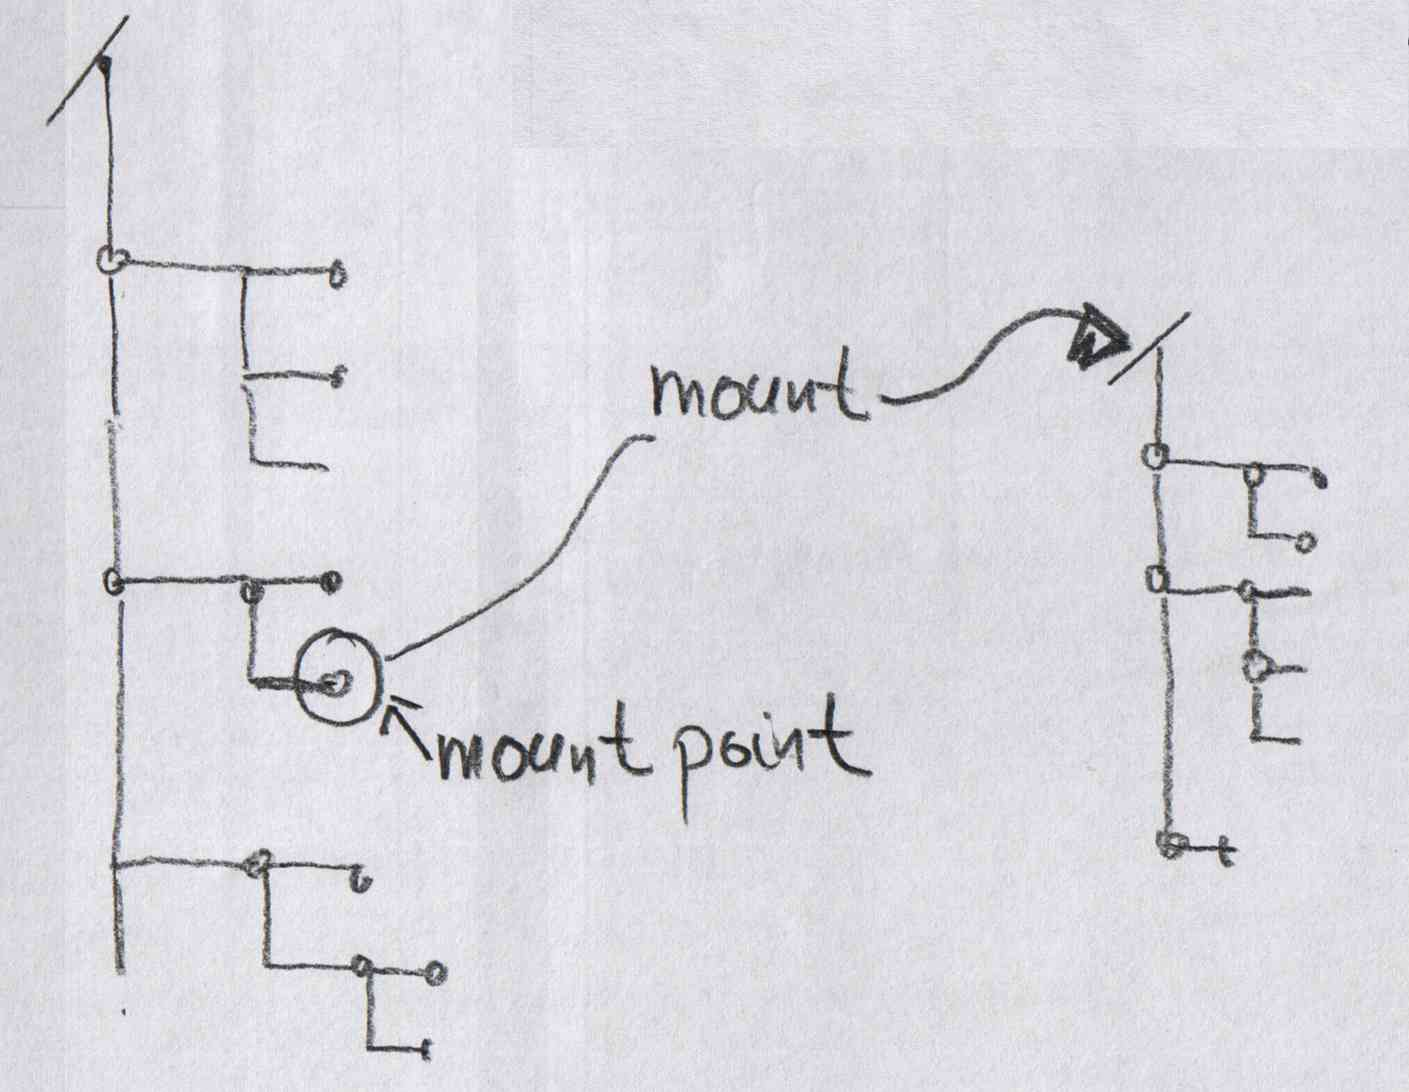
\includegraphics[height=3.5cm]{mount.jpg}
  \begin{textblock}{150}(58,40)
   \begin{itemize}
    \item \cod{mount {\em /dev/mmcblk0p1} %\textbackslash \\
    {\em mountPoint}}
	\item \cod{umount {\em mountPoint}}
   \end{itemize}
  \end{textblock}
  \remark{{\em mountPoint} sieht wie ein normales Verzeichnis aus}
\end{frame}

\begin{frame}{\cod{sshfs user@target:{\em path} {\em mountPoint}}}{via \cod{ssh}}
 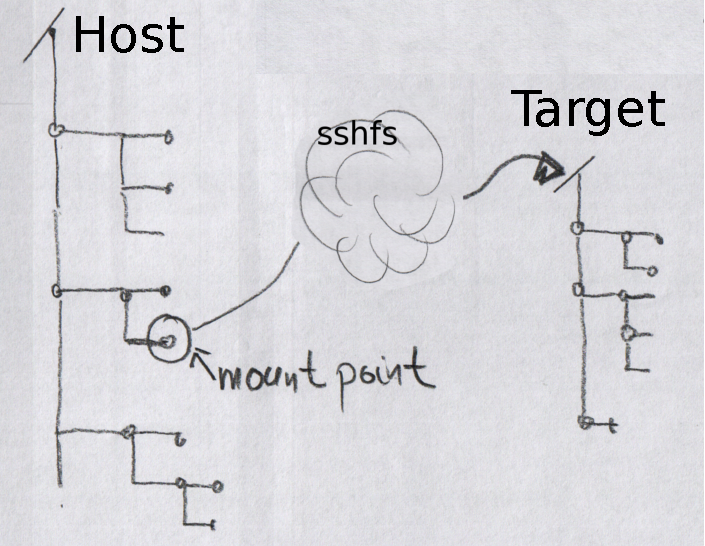
\includegraphics[height=3.5cm]{sshfs.pdf}
   \begin{textblock}{150}(58,40)
   \begin{itemize}
    \item \cod{sshfs user@target:{\em path} {\em mountPoint}}
	\begin{itemize}
     \item braucht \cod{ssh}
	\end{itemize}
	\item \cod{fusermount -u {\em mountPoint}}
	\begin{itemize}
	 \item umount
	\end{itemize}
   \end{itemize}
  \end{textblock}
  \remark{{\em mountPoint} Sieht wie ein normales Verzeichnis aus}
\end{frame}

%\section{Cross development}
%\begin{frame}{Crossdevelopment}
 \begin{itemize}
  \item Development
  \begin{itemize}
   \item Wo sind die Files
  \end{itemize}
  \item CrossDevelopment
  \begin{itemize}
   \item Wo sind die Files
  \end{itemize}
 \end{itemize}
\end{frame}

\subsection{Development}
\begin{frame}{Development}{noch nicht Cross}
 \begin{itemize}
  \item Source file \cod{src/hello-world-c.c}
  \begin{itemize}
   \item C
   \item POSIX
  \end{itemize}
  unabh�ngig von Platform
  \item Object file (Maschinencode) \cod{hello-world-c.o}
  \begin{itemize}
   \item erzeugt mit: \cod{gcc -c ../src/hello-world-c.c -o hello-world-c.o}
   \item Maschinencode: 
   \begin{itemize}
    \item \cod{file hello-world-c.o} 
    \item \cod{objdump -d hello-world-c.o}
   \end{itemize}
  \end{itemize}
  \item Executable file \cod{hello-world-c}
  \begin{itemize}
   \item \cod{gcc  hello-world-c.o -o hello-world-c}
   \item Maschinencode:
   \begin{itemize}
    \item \cod{file hello-world-c} 
    \item \cod{objdump -d hello-world-c}
   \end{itemize}
  \end{itemize}
 \end{itemize}
\end{frame}

\begin{frame}{Was es braucht ?}{Files}
 \begin{itemize}
  \item Source file
  \begin{itemize}
   \item wo ist der {\em include file} \cod{stdio.h}
  \end{itemize}
  \item Object File
  \begin{itemize}
   \item \cod{nm hello-world-c.o}
   \item wo ist \cod{puts}
  \end{itemize}
  \item Executable
  \begin{itemize}
  \item \cod{nm hello-world-c}
  \item \cod{ldd hello-world-c}
  \item wo sind die Bibliotheken
  \end{itemize}
 \end{itemize}
\end{frame}

\begin{frame}{Wo sind die Files ?}{irgendwo in einem Unterverzeichnis von {\Huge\tt /}}
 \begin{itemize}
  \item Include Files \cod{gcc -c -v ../src/hello-world-c.c -o hello-world-c.o}
  \begin{itemize}
   \item \cod{stdio.h} ?
   \item \cod{stddef.h} ? 
  \end{itemize}
  \item Bibliotheken
  \begin{itemize}
   \item z.B. \cod{libc.so}
  \end{itemize}
 \end{itemize}
\end{frame}

\begin{frame}{Development}{der Normalfall}
 \begin{itemize}
  \item Host==Target
  \item root Host==root Target
 \end{itemize}
\end{frame}

\subsection{CrossDevelopment}

\begin{frame}{CrossDevelopment}
 \begin{itemize}
  \item immer noch POSIX
  \item Host!=Target
 \end{itemize}
\end{frame}

\begin{frame}{Verzeichnisstruktur}{\host}
 \dirtree{%
  .1 2-unix-use \DTcomment{somewhere on the host}.
  .2 target-root \DTcomment{different possibilities}.
  .2 config.
  .3 Makefile \DTcomment{for making \target executables}.
  .2 src  \DTcomment{c,c++}.
  .2 tc   \DTcomment{toolchain}.
  .2 {\bf work} \DTcomment{connected with \target {\em current dir}}.
 }
\end{frame}

\begin{frame}{CrossDevelopment}{Target \host:}
 \begin{itemize}
  \item Makefile
  \begin{itemize}
   \item \cod{PREFFIX=}
  \end{itemize}
  \item \cod{target-root}
  \begin{itemize}
   \item \cod{ln -s / target-root}
  \end{itemize}
 \end{itemize}
 \remark{un�blich !}
\end{frame}

\begin{frame}{CrossDevelopment}{Target \target}
 \begin{itemize}
  \item Makefile
  \begin{itemize}
   \item \cod{PREFFIX=../tc/bin/arm-linux-gnueabihf-}
  \end{itemize}
  \item \cod{target-root}
  \begin{itemize}
   \item \cod{sshfs debian@192.168.7.2:/ target-root}
  \end{itemize}
 \end{itemize}
\end{frame}

\begin{frame}{Verzeichnisstruktur}{\target}
 \dirtree{%
  .1 /.
  .2 home.
  .3 debian \DTcomment{user}.
  .4 {\bf work}.
 }
\end{frame}

\subsection{Aufgaben}
\begin{frame}{The big Picture}
 \begin{itemize}
  \item Source File: \cod{hello-world-c.c}
  \item falls es nicht klapt ?
  \begin{itemize}
   \item wo ist der File ?
  \end{itemize}
 \end{itemize}
\end{frame}

\begin{frame}{Development}{\cod{hello-world-c.c}}
\hspace*{-8mm}
{
\begin{tabular}{llllll}
 Host & Target & OS & Toolchain & Verbindung & Bemerkungen\\
 \hline
 \targetS & \targetS & Debian & mitgeliefert&&\\
 \host   & \targetS & Debian & \cod{\tiny gcc-7.2.0-arm-64bit.tar.bz2} & sshfs\\
 \host   & \targetS & minimal & \cod{\tiny gcc-7.2.0-arm-64bit.tar.gz} & SD-Card  &sp�ter\\
 \host   & \targetS & minimal & \cod{\tiny gcc-7.2.0-arm-64bit.tar.gz} & curlftpfs&sp�ter\\
\end{tabular}
}
\end{frame}

%\begin{frame}{Crossdevelopment}{\cod{hello-world-c.c}}
%\begin{itemize}
% \item Target \target Debian
% \item Host \host:
% \begin{itemize}
%  \item \cod{target-root}
%  \item \cod{sshfs}
% \end{itemize} 
% \end{itemize} 
%\end{frame}
%
%\begin{frame}{Crossdevelopment}{\cod{hello-world-c.c}}
% \begin{itemize}
% \item Target \target minimal \cod{mmc0} 
% \item Host \host\ \cod{target-root}:
% \begin{itemize}
%  \item toolchain:
%  \begin{itemize}
%   \item \cod{gcc-6.2.0-arm-64bit.tar.gz} in 
%   \url{sourceforge.net/projects/fhnw-tinl/files}
%  \end{itemize}
%  \item SD-Karte ein-\& ausstecken
%  \item Kopie 
%  \item \cod{curlftpfs}
%  \begin{itemize}
%   \item basiert auf \cod{ftp} 
%  \end{itemize}
% \end{itemize} 
% \end{itemize} 
%\end{frame}
%
%\begin{frame}{Vorbereitung}
% \begin{itemize}
%  \item Verbindung mit \target via \cod{ssh}
%%  \item upgrade \cod{pacman -Suy}
%%  \item {\em user} auf \target \cod{useradd}
%  \item Installation {\em toolchain} auf \host
%  
%  {\tiny\url{sourceforge.net/projects/fhnw-tinl/files/}}
% \end{itemize}
%\end{frame}
%
%\begin{frame}{Verbindung}{mit \target Debian}
% \begin{itemize}
%  \item \cod{ssh} f�r die Ausf�hrung der Programme
%  \item {\em mount} Varianten
%  \begin{itemize}
%   \item \host auf \target 
%  \end{itemize}
%  \item Kopiere  {\em executable} auf \target 
%   \begin{itemize}
%    \item \cod{scp} secure copy
%    \item \cod{scp {\em executable} user@target:}
%   \end{itemize}
% \end{itemize}
%\end{frame}
%
%\begin{frame}{Programme}{auf \target}
% \begin{itemize}
%  \item \c Programme:, \cod{hello-world-c.c} 
%  \item \cpp Programme \cod{hello-world-cpp.cc}, \cod{primes.cc} 
%  \remark{Toolchain funktioniert f�r \cpp noch nicht}
% \end{itemize}
%\end{frame}

%\begin{frame}{Verzeichnisstruktur}{\host$\leftrightarrow$ \target}
% \begin{block}{Host} 
% \dirtree{%
%  .1 2-unix-use \DTcomment{somewhere on the host}.
%  .2 config.
%  .3 Makefile \DTcomment{for making \target executables}.
%  .2 src  \DTcomment{c,c++}.
%  .2 tc   \DTcomment{normally toolchain}.
%  .2 {\bf work} \DTcomment{connected with \target {\em current dir}}.
% }
% \end{block}
% \begin{block}{\target} 
% \dirtree{%
%  .1 user \DTcomment{somewhere on the \target}.
%  .2 {\bf work} \DTcomment{connected with \host {\em current dir}}.
% }
% \end{block}
%\end{frame}




\end{document}

